% Biên dịch: python report2/build.py (sinh lại số liệu từ results/, rồi chạy XeLaTeX hai lần).
% Mọi con số trong bài đến từ report2/generated/*.tex do report2/make_assets.py sinh ra.
\documentclass[11pt,a4paper]{article}

\usepackage{fontspec}
\setmainfont{Times New Roman}
\usepackage[vietnamese]{babel}
\usepackage[margin=2.2cm]{geometry}
\usepackage{graphicx}
\usepackage{booktabs}
\usepackage{amsmath}
\usepackage{amssymb}
\usepackage{caption}
\usepackage[hidelinks]{hyperref}
\usepackage{xcolor}

\graphicspath{{generated/}}
\captionsetup{font=small,labelfont=bf}
\setlength{\parskip}{0.4em}
\setlength{\parindent}{0pt}

\newif\ifshowtodo\showtodofalse
\newcommand{\todo}[1]{\ifshowtodo{\color{red}\small[TODO: #1]}\fi}

\newcommand{\probebestname}{ResNet18}
\newcommand{\probebestcv}{99{,}74\%}
\newcommand{\probebestheld}{99{,}37\%}
\newcommand{\probeworstname}{VGG11-BN}
\newcommand{\probeworstcv}{99{,}32\%}
\newcommand{\lightname}{MobileNetV3-Small}
\newcommand{\lightparams}{2{,}5}
\newcommand{\lightcv}{99{,}63\%}
\newcommand{\lightms}{11}
\newcommand{\heavyname}{VGG11-BN}
\newcommand{\heavyparams}{132{,}9}
\newcommand{\heavycv}{99{,}32\%}
\newcommand{\heavyms}{50}
\newcommand{\paramratio}{52}
\newcommand{\ftacc}{99{,}79\%}
\newcommand{\ftprecision}{99{,}82\%}
\newcommand{\ftrecall}{99{,}80\%}
\newcommand{\ftfone}{99{,}80\%}
\newcommand{\ftperfect}{30}
\newcommand{\ftclasses}{32}
\newcommand{\fterrors}{1}
\newcommand{\probeacc}{99{,}37\%}
\newcommand{\probeperfect}{28}
\newcommand{\bestepoch}{5}
\newcommand{\epochseconds}{45}
\newcommand{\epochs}{6}
\newcommand{\firstepochacc}{96{,}44\%}
\newcommand{\classicalcv}{98{,}85\%}
\newcommand{\cnngain}{0{,}89}
\newcommand{\nclasses}{32}


\addto\captionsvietnamese{\renewcommand{\refname}{Tài liệu tham khảo}}

\title{\vspace{-1.5cm}Phân lớp lá cây trên bộ dữ liệu Flavia bằng mạng nơ-ron tích chập\\
\large Học chuyển giao với ResNet18, MobileNetV3 và VGG11}
\author{Học viên thực hiện: Võ Hoàng Khang \quad MSHV: 25C01034\\[0.3em]
\small Mã nguồn: \url{https://github.com/vo-hoang-kh4ng/Leaf-Segmentation}}
\date{\today}

\begin{document}
\maketitle
\vspace{-0.8cm}

\begin{abstract}
\noindent
Báo cáo giải lại bài toán phân lớp \nclasses{} loài lá cây trên bộ dữ liệu Flavia (1907 ảnh) bằng
mạng nơ-ron tích chập, thay cho đặc trưng thủ công của bài tập trước. Ba kiến trúc tiền huấn luyện
trên ImageNet được so sánh ở hai chế độ sử dụng: đóng băng toàn bộ backbone và chỉ huấn luyện một
bộ phân lớp tuyến tính, hoặc tinh chỉnh (fine-tune) khối tích chập cuối. Toàn bộ thí nghiệm dùng
đúng phép chia dữ liệu và giao thức đánh giá của bài tập trước, nên các con số so sánh được trực
tiếp. Kết quả chính: với backbone \emph{đóng băng hoàn toàn}, \probebestname{} đã đạt \probebestcv{}
(kiểm định chéo 5 phần), cao hơn \cnngain{} điểm so với \classicalcv{} của quy trình đặc trưng thủ
công; fine-tune nâng độ chính xác trên tập kiểm tra giữ lại lên \ftacc{}, chỉ còn \fterrors{} ảnh bị
phân lớp sai trên 477 ảnh. Hai quan sát đáng chú ý: số tham số không dự báo chất lượng biểu diễn
chuyển giao (\lightname{} với \lightparams{} triệu tham số vượt \heavyname{} với \heavyparams{}
triệu), và phần lớn thành tích đến từ biểu diễn ImageNet có sẵn chứ không từ quá trình huấn luyện
lại trên ảnh lá.
\end{abstract}

\section{Giới thiệu}

Bài tập trước giải bài toán Flavia bằng đặc trưng thủ công: phân đoạn lá, trích xuất bốn nhóm đặc
trưng (hình dạng, màu sắc, kết cấu, gân lá) do con người thiết kế, rồi phân lớp bằng SVM, đạt
\classicalcv{}. Cách làm đó đòi hỏi hiểu biết chuyên môn ở từng bước: phải biết rằng độ răng cưa
của mép lá mang thông tin phân loài thì mới nghĩ ra đặc trưng đo nó.

Mạng nơ-ron tích chập thay đổi vị trí của tri thức chuyên môn: thay vì thiết kế đặc trưng, ta thiết
kế kiến trúc và để mạng tự học biểu diễn từ dữ liệu~\cite{lecun1998}. Trở ngại là mạng sâu cần rất
nhiều dữ liệu, trong khi Flavia chỉ có 1907 ảnh. Lời giải tiêu chuẩn cho tình huống này là
\emph{học chuyển giao}: lấy mạng đã huấn luyện trên ImageNet~\cite{deng2009} với hơn một triệu ảnh,
rồi tái sử dụng biểu diễn đó cho bài toán mới.

Báo cáo trả lời ba câu hỏi:
\begin{itemize}
  \item Biểu diễn học từ ImageNet có sẵn sàng tách được 32 loài lá hay không, khi \emph{không} huấn
        luyện lại gì trong mạng?
  \item Ba kiến trúc với độ phức tạp chênh nhau \paramratio{} lần khác nhau thế nào trên bài toán này?
  \item Tinh chỉnh mạng thêm được bao nhiêu so với việc chỉ dùng mạng như bộ trích đặc trưng?
\end{itemize}

\section{Dữ liệu và giao thức đánh giá}

Bộ dữ liệu giữ nguyên như bài tập trước: Flavia, 1907 ảnh JPEG $1600\times1200$, \nclasses{} loài,
mỗi lớp 50--77 ảnh, nhãn mã hoá trong số hiệu tên tệp.

Điểm then chốt về phương pháp: \textbf{phép chia dữ liệu, hạt giống ngẫu nhiên và cách đánh giá được
giữ y hệt bài tập trước} --- kiểm định chéo phân tầng 5 phần trên toàn bộ 1907 ảnh, cộng một tập
kiểm tra giữ lại 25\% (477 ảnh) với cùng hạt giống. Nếu đổi cách chia, con số của CNN sẽ không còn
so sánh được với con số của đặc trưng thủ công, và toàn bộ phần so sánh trong Bảng~\ref{tab:comparison}
sẽ mất ý nghĩa.

Một khác biệt lớn so với bài trước: \textbf{quy trình CNN không cần bước phân đoạn}. Đặc trưng thủ
công bắt buộc phải tách lá khỏi nền trước, vì diện tích hay độ đặc chỉ định nghĩa được trên một vùng
đã phân đoạn. CNN nhận thẳng ảnh màu, chỉ cần đưa về kích thước $224\times224$ và chuẩn hoá theo
thống kê của ImageNet để khớp với phân phối dữ liệu mà backbone đã được huấn luyện.

Ảnh được đưa về $224\times224$ bằng phép co giãn trực tiếp chứ không cắt giữa: phép cắt sẽ xén mất
phần chóp của những chiếc lá dài, mà chóp lá lại là chi tiết phân biệt nhiều loài.

\section{Cơ sở lý thuyết}

\subsection{Mạng tích chập}

Tầng tích chập trượt một bộ lọc nhỏ trên toàn ảnh và dùng chung một bộ trọng số cho mọi vị trí. Hai
hệ quả quan trọng: số tham số giảm mạnh so với tầng kết nối đầy đủ, và đặc trưng học được có tính
bất biến tịnh tiến --- một mép lá răng cưa được nhận ra bất kể nó nằm ở đâu trong ảnh. Xếp chồng
nhiều tầng tạo ra hệ thống phân cấp: tầng đầu phản ứng với biên và vùng màu, các tầng sau tổ hợp
chúng thành hoạ tiết rồi thành bộ phận của vật thể. AlexNet~\cite{krizhevsky2012} là công trình đưa
kiến trúc này thành phương pháp thống trị trong thị giác máy tính.

\subsection{Ba kiến trúc được so sánh}

\textbf{VGG11}~\cite{simonyan2015} theo đuổi sự đơn giản: chỉ dùng bộ lọc $3\times3$ xếp chồng, xen
kẽ với phép gộp cực đại. Hai bộ lọc $3\times3$ liên tiếp có cùng vùng tiếp nhận với một bộ lọc
$5\times5$ nhưng ít tham số hơn và có thêm một phi tuyến. Nhược điểm là khối kết nối đầy đủ ở cuối
rất nặng: riêng phần này chiếm phần lớn trong \heavyparams{} triệu tham số của mạng.

\textbf{ResNet18}~\cite{he2016} giải quyết hiện tượng mạng càng sâu thì càng khó huấn luyện. Thay vì
học trực tiếp ánh xạ $H(x)$, mỗi khối học phần dư $F(x) = H(x) - x$ và cộng lại qua kết nối tắt:
\[
y = F(x, \{W_i\}) + x .
\]
Kết nối tắt tạo đường truyền gradient không bị suy giảm qua nhiều tầng, nhờ đó huấn luyện được mạng
sâu hàng chục đến hàng trăm tầng.

\textbf{MobileNetV3-Small}~\cite{howard2019} được thiết kế cho thiết bị tính toán hạn chế. Ý tưởng
cốt lõi là tách tích chập thường thành \emph{depthwise} (lọc riêng từng kênh) và \emph{pointwise}
($1\times1$ để trộn kênh), giảm chi phí tính toán khoảng 8--9 lần với bộ lọc $3\times3$. Mạng bổ
sung khối Squeeze-and-Excitation để tái trọng số các kênh và hàm kích hoạt h-swish; kiến trúc được
tìm bằng tìm kiếm tự động.

\subsection{Học chuyển giao}

Các tầng đầu của mạng huấn luyện trên ImageNet học những thứ rất tổng quát --- biên, góc, đốm màu,
hoạ tiết --- và những thứ này đúng với mọi ảnh tự nhiên, không riêng gì 1000 lớp của ImageNet. Vì
vậy có thể giữ nguyên chúng và chỉ thay phần đầu ra. Báo cáo so sánh hai mức độ tái sử dụng:

\begin{itemize}
  \item \textbf{Backbone đóng băng (linear probe).} Bỏ tầng phân lớp của ImageNet, dùng mạng như một
        hàm trích đặc trưng cố định, rồi huấn luyện một bộ phân lớp tuyến tính (hồi quy logistic) lên
        trên. Không một trọng số nào trong mạng thay đổi. Cách này trả lời câu hỏi: thông tin phân
        biệt loài đã có sẵn trong biểu diễn ImageNet chưa?
  \item \textbf{Tinh chỉnh (fine-tune).} Mở khoá khối tích chập cuối (\texttt{layer4} của ResNet18)
        cùng tầng phân lớp mới, cho phép mạng điều chỉnh các đặc trưng bậc cao cho phù hợp với lá cây.
\end{itemize}

\section{Phương pháp thực nghiệm}

\subsection{Trích đặc trưng với backbone đóng băng}

Mỗi ảnh được đưa qua backbone một lần, thu được vectơ đặc trưng (512 chiều với ResNet18, 576 với
MobileNetV3, 4096 với VGG11 lấy ở tầng kết nối đầy đủ thứ hai). Toàn bộ 1907 vectơ được lưu lại,
nên các thí nghiệm sau chỉ làm việc trên ma trận đặc trưng thay vì đọc lại ảnh --- cùng nguyên tắc
với bài tập trước, nơi bước trích đặc trưng tốn kém còn bước phân lớp gần như miễn phí.

Bộ phân lớp là hồi quy logistic đa lớp, có chuẩn hoá z-score đặt bên trong quy trình huấn luyện để
chỉ được ước lượng trên phần huấn luyện của mỗi lần chia, tránh rò rỉ dữ liệu.

\subsection{Tinh chỉnh ResNet18}

Chỉ \texttt{layer4} và tầng phân lớp mới được huấn luyện; các tầng còn lại bị đóng băng. Với 1430
ảnh huấn luyện, mở khoá toàn mạng sẽ dẫn tới quá khớp, và trên CPU cũng quá chậm.

Hai tốc độ học khác nhau được dùng cho hai nhóm tham số: tầng phân lớp khởi tạo ngẫu nhiên nên cần
bước lớn ($10^{-3}$), còn \texttt{layer4} xuất phát từ một nghiệm đã tốt nên chỉ cần bước nhỏ
($10^{-4}$). Dùng chung một tốc độ học sẽ hoặc phá hỏng khối tiền huấn luyện, hoặc làm tầng phân lớp
học quá chậm. Thuật toán tối ưu là AdamW, hàm mất mát là entropy chéo, \epochs{} epoch, mỗi epoch
khoảng \epochseconds{} giây trên CPU 16 luồng.

\textbf{Tăng cường dữ liệu} chỉ áp dụng cho tập huấn luyện, và được giữ ở mức vừa phải: lật ngang,
lật dọc, xoay ngẫu nhiên tối đa $20^\circ$ (lấp nền trắng cho khớp nền Flavia), thay đổi nhẹ độ sáng
và độ tương phản. Lá trên máy quét không có hướng chuẩn nên lật và xoay là phép biến đổi bảo toàn
nhãn. Ngược lại, thay đổi màu bị giữ ở biên độ nhỏ vì màu sắc thực sự mang thông tin phân loài:
bài tập trước đo được nhóm đặc trưng màu đóng góp hơn 11 điểm phần trăm. Biến dạng màu mạnh sẽ xoá
mất tín hiệu chứ không tạo thêm tính bất biến hữu ích.

\section{Kết quả}

\subsection{So sánh ba backbone đóng băng}

Bảng~\ref{tab:backbones} trình bày kết quả. Điều đáng chú ý đầu tiên: \textbf{cả ba mạng đều vượt
\classicalcv{} của quy trình đặc trưng thủ công, dù không một trọng số nào trong mạng được huấn
luyện trên ảnh lá}. Biểu diễn học từ ImageNet đã đủ để tách 32 loài lá bằng một mặt phẳng tuyến tính.

\begin{table}[t]
\centering
\caption{Ba backbone tiền huấn luyện ImageNet, đóng băng hoàn toàn, chỉ huấn luyện một bộ phân lớp tuyến tính phía trên. Giao thức đánh giá trùng khớp với bài tập 1: kiểm định chéo phân tầng 5 phần trên 1907 ảnh và tập kiểm tra giữ lại 25\%. Thời gian suy luận đo trên CPU 16 luồng.}
\label{tab:backbones}
\small
\begin{tabular}{l r r r r r}
\toprule
Backbone & Tham số (M) & Số chiều & Kiểm định chéo & Giữ lại & ms/ảnh \\
\midrule
ResNet18 & 11{,}7 & 512 & \textbf{0{,}9974} & 0{,}9937 & 17{,}9 \\
MobileNetV3-Small & 2{,}5 & 576 & 0{,}9963 & 0{,}9937 & 10{,}4 \\
VGG11-BN & 132{,}9 & 4096 & 0{,}9932 & 0{,}9958 & 49{,}8 \\
\bottomrule
\end{tabular}
\end{table}

\begin{table}[t]
\centering
\caption{So sánh với bài tập 1 trên cùng bộ dữ liệu, cùng phép chia phân tầng và cùng hạt giống ngẫu nhiên. Cấu hình fine-tune chỉ có một con số vì nó được huấn luyện trên phần huấn luyện của phép chia giữ lại, không chạy kiểm định chéo (chi phí tính toán).}
\label{tab:comparison}
\small
\begin{tabular}{l r r}
\toprule
Phương pháp & Kiểm định chéo & Tập giữ lại \\
\midrule
Đặc trưng thủ công + SVM (bài tập 1) & 0{,}9885 & 0,9895 \\
ResNet18 đóng băng + phân lớp tuyến tính & 0{,}9974 & 0{,}9937 \\
ResNet18 fine-tune (mở khoá block cuối) & --- & 0{,}9979 \\
\bottomrule
\end{tabular}
\end{table}

\begin{table}[t]
\centering
\caption{Toàn bộ các loài không đạt F1 = 1,00 với mô hình ResNet18 fine-tune. Những loài còn lại đều đạt precision và recall bằng 1,00.}
\label{tab:perclass}
\small
\begin{tabular}{l r r r r}
\toprule
Loài & Precision & Recall & F1 & Số mẫu \\
\midrule
Canadian poplar & 1{,}000 & 0{,}938 & 0{,}968 & 16 \\
camphortree & 0{,}941 & 1{,}000 & 0{,}970 & 16 \\
\bottomrule
\end{tabular}
\end{table}


\textbf{Số tham số không dự báo chất lượng biểu diễn.} \lightname{} chỉ có \lightparams{} triệu
tham số, nhỏ hơn \heavyname{} \paramratio{} lần, nhưng đạt \lightcv{} so với \heavycv{}, đồng thời
nhanh hơn 5 lần (\lightms{} ms so với \heavyms{} ms mỗi ảnh trên CPU). Kiến trúc hiện đại với tích
chập tách được khai thác tham số hiệu quả hơn hẳn kiểu xếp chồng kết nối đầy đủ của VGG.

Tuy nhiên, chênh lệch giữa các mạng rất nhỏ nên cần kiểm định trước khi xếp hạng. Kiểm định $t$ ghép
cặp trên cùng các phần kiểm định chéo cho thấy \textbf{chỉ một cặp đạt ý nghĩa thống kê}:
\probebestname{} hơn \probeworstname{} ($p = 0{,}035$). Hai cặp còn lại có $p = 0{,}15$--$0{,}18$,
tức chưa đủ cơ sở kết luận mạng nào hơn. Đây là cùng kỷ luật đã rút ra ở bài tập trước: với mức
chênh lệch dưới một điểm phần trăm, xếp hạng theo chữ số thập phân là diễn giải nhiễu.

\subsection{Tinh chỉnh}

Hình~\ref{fig:curve} cho thấy quá trình huấn luyện. Ngay sau epoch đầu tiên, độ chính xác trên tập
kiểm tra đã đạt \firstepochacc{} --- hệ quả trực tiếp của việc xuất phát từ trọng số ImageNet thay
vì khởi tạo ngẫu nhiên. Mô hình tốt nhất xuất hiện ở epoch \bestepoch{} với \ftacc{}. Hàm mất mát
trên tập kiểm tra giảm đều và không bật lên, nghĩa là với số epoch này mô hình chưa quá khớp.

\begin{figure}[t]
  \centering
  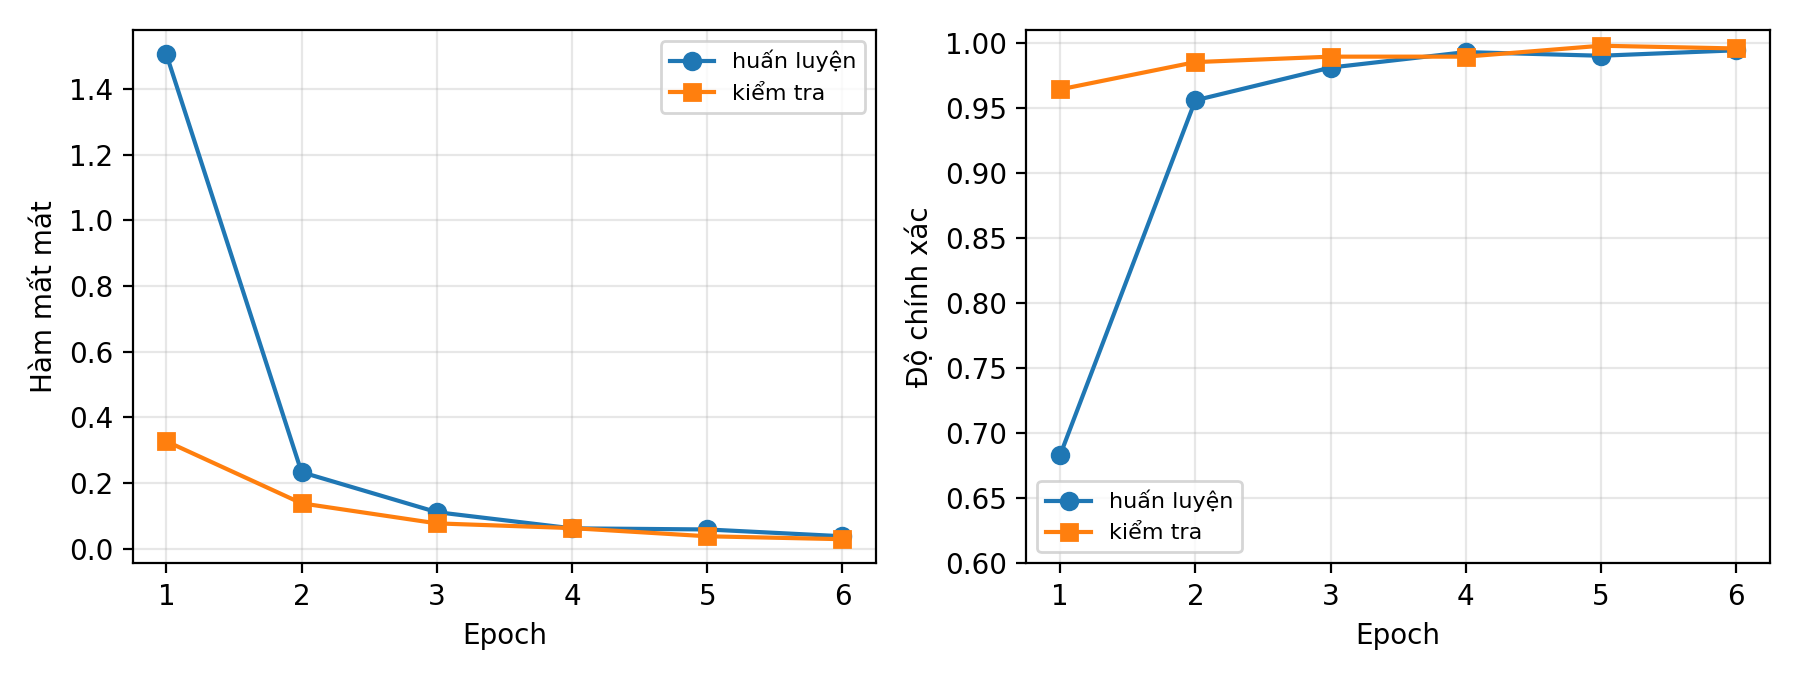
\includegraphics[width=\linewidth]{training_curve.png}
  \caption{Quá trình tinh chỉnh ResNet18 qua \epochs{} epoch.}
  \label{fig:curve}
\end{figure}

So với cùng mạng ở chế độ đóng băng (\probeacc{} trên cùng tập kiểm tra), tinh chỉnh nâng kết quả
lên \ftacc{}. Cần thận trọng khi diễn giải: trên 477 ảnh, khoảng cách này tương ứng chỉ vài ảnh, nên
nó cho thấy một xu hướng hợp lý chứ không phải một kết luận chắc chắn về mặt thống kê.

\subsection{Ma trận nhầm lẫn, precision và recall}

Với \nclasses{} lớp có kích thước không đều, riêng độ chính xác tổng thể là chưa đủ: một loài nhỏ có
thể bị sai toàn bộ mà con số tổng vẫn gần như không đổi. Vì vậy kết quả được báo cáo theo từng lớp.

Mô hình tinh chỉnh đạt macro precision \ftprecision{}, macro recall \ftrecall{} và macro F1
\ftfone{}. \textbf{\ftperfect{}/\ftclasses{} loài đạt F1 bằng 1,00}, tức precision và recall đều
tuyệt đối. Bảng~\ref{tab:perclass} liệt kê toàn bộ các loài còn lại, và Hình~\ref{fig:pr} biểu diễn
precision cùng recall của mọi loài.

\begin{figure}[t]
  \centering
  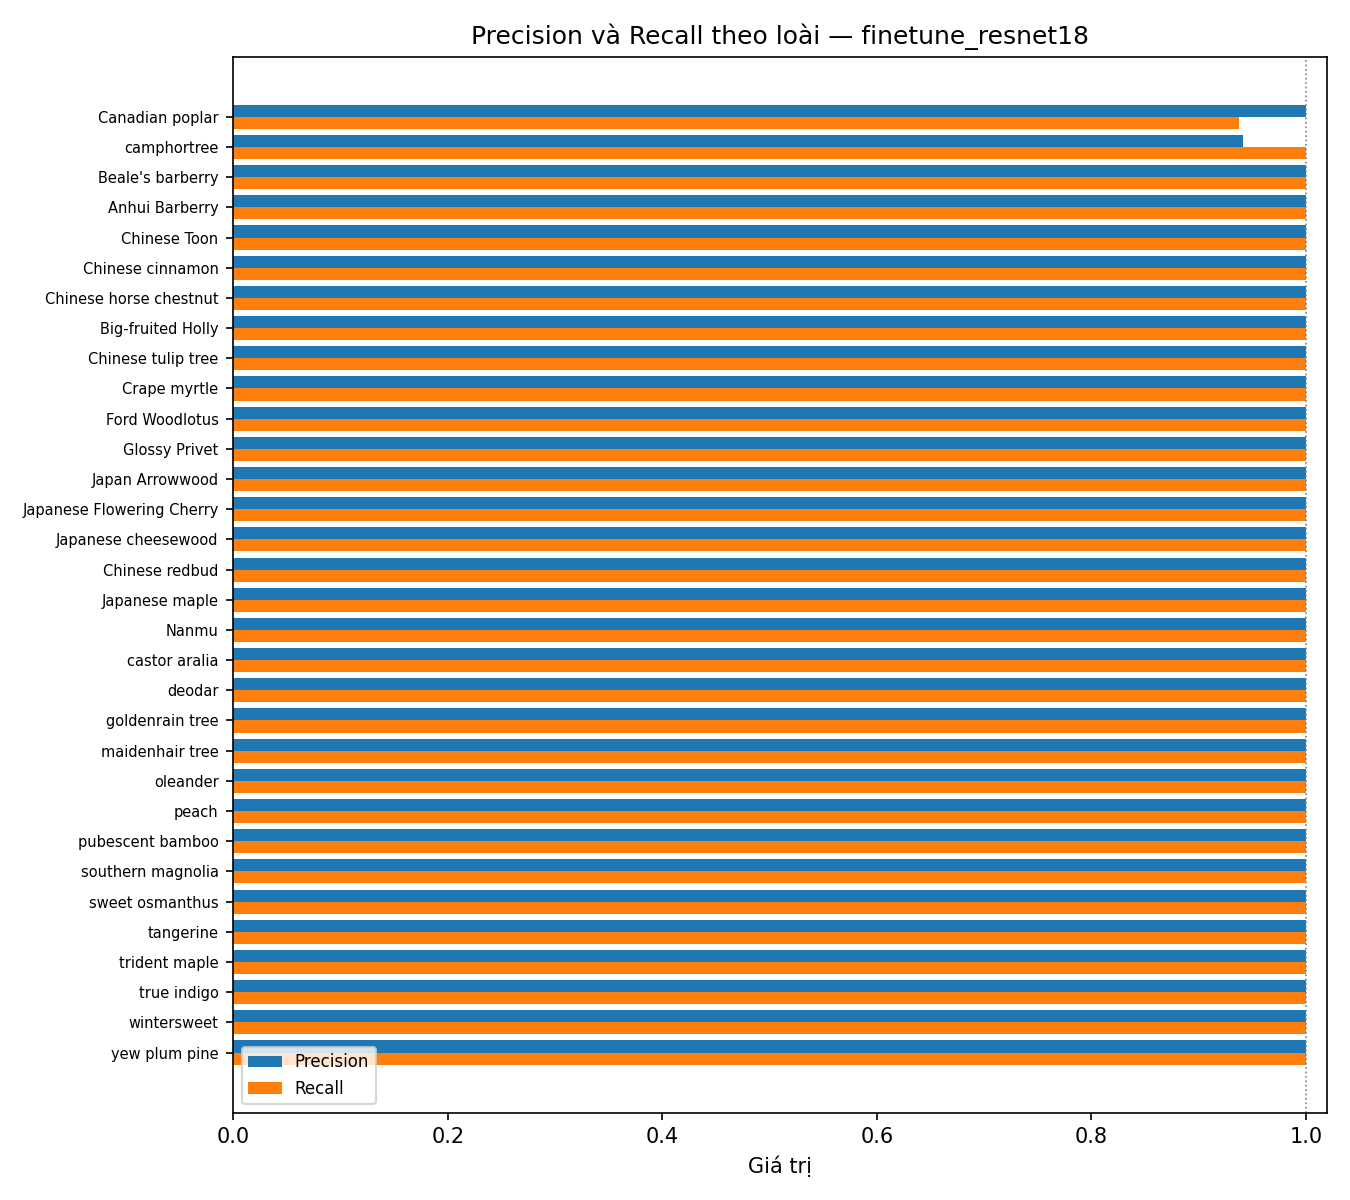
\includegraphics[width=0.78\linewidth]{precision_recall.png}
  \caption{Precision và recall theo từng loài trên tập kiểm tra giữ lại, sắp xếp theo F1.}
  \label{fig:pr}
\end{figure}

Ma trận nhầm lẫn ở Hình~\ref{fig:confusion} cho thấy toàn bộ khối lượng nằm trên đường chéo, ngoại
trừ đúng \fterrors{} ô: một ảnh \emph{Canadian poplar} bị nhận thành \emph{camphortree}. Chính cặp
này cũng xuất hiện ở mô hình đóng băng, bên cạnh hai ảnh \emph{peach} bị nhận thành \emph{Anhui
Barberry} mà việc tinh chỉnh đã sửa được. Với chỉ một mẫu sai, không thể kết luận gì về nguyên nhân;
cần nhiều dữ liệu kiểm tra hơn mới nói được đây là nhầm lẫn có hệ thống hay chỉ là một ảnh biên.

\begin{figure}[t]
  \centering
  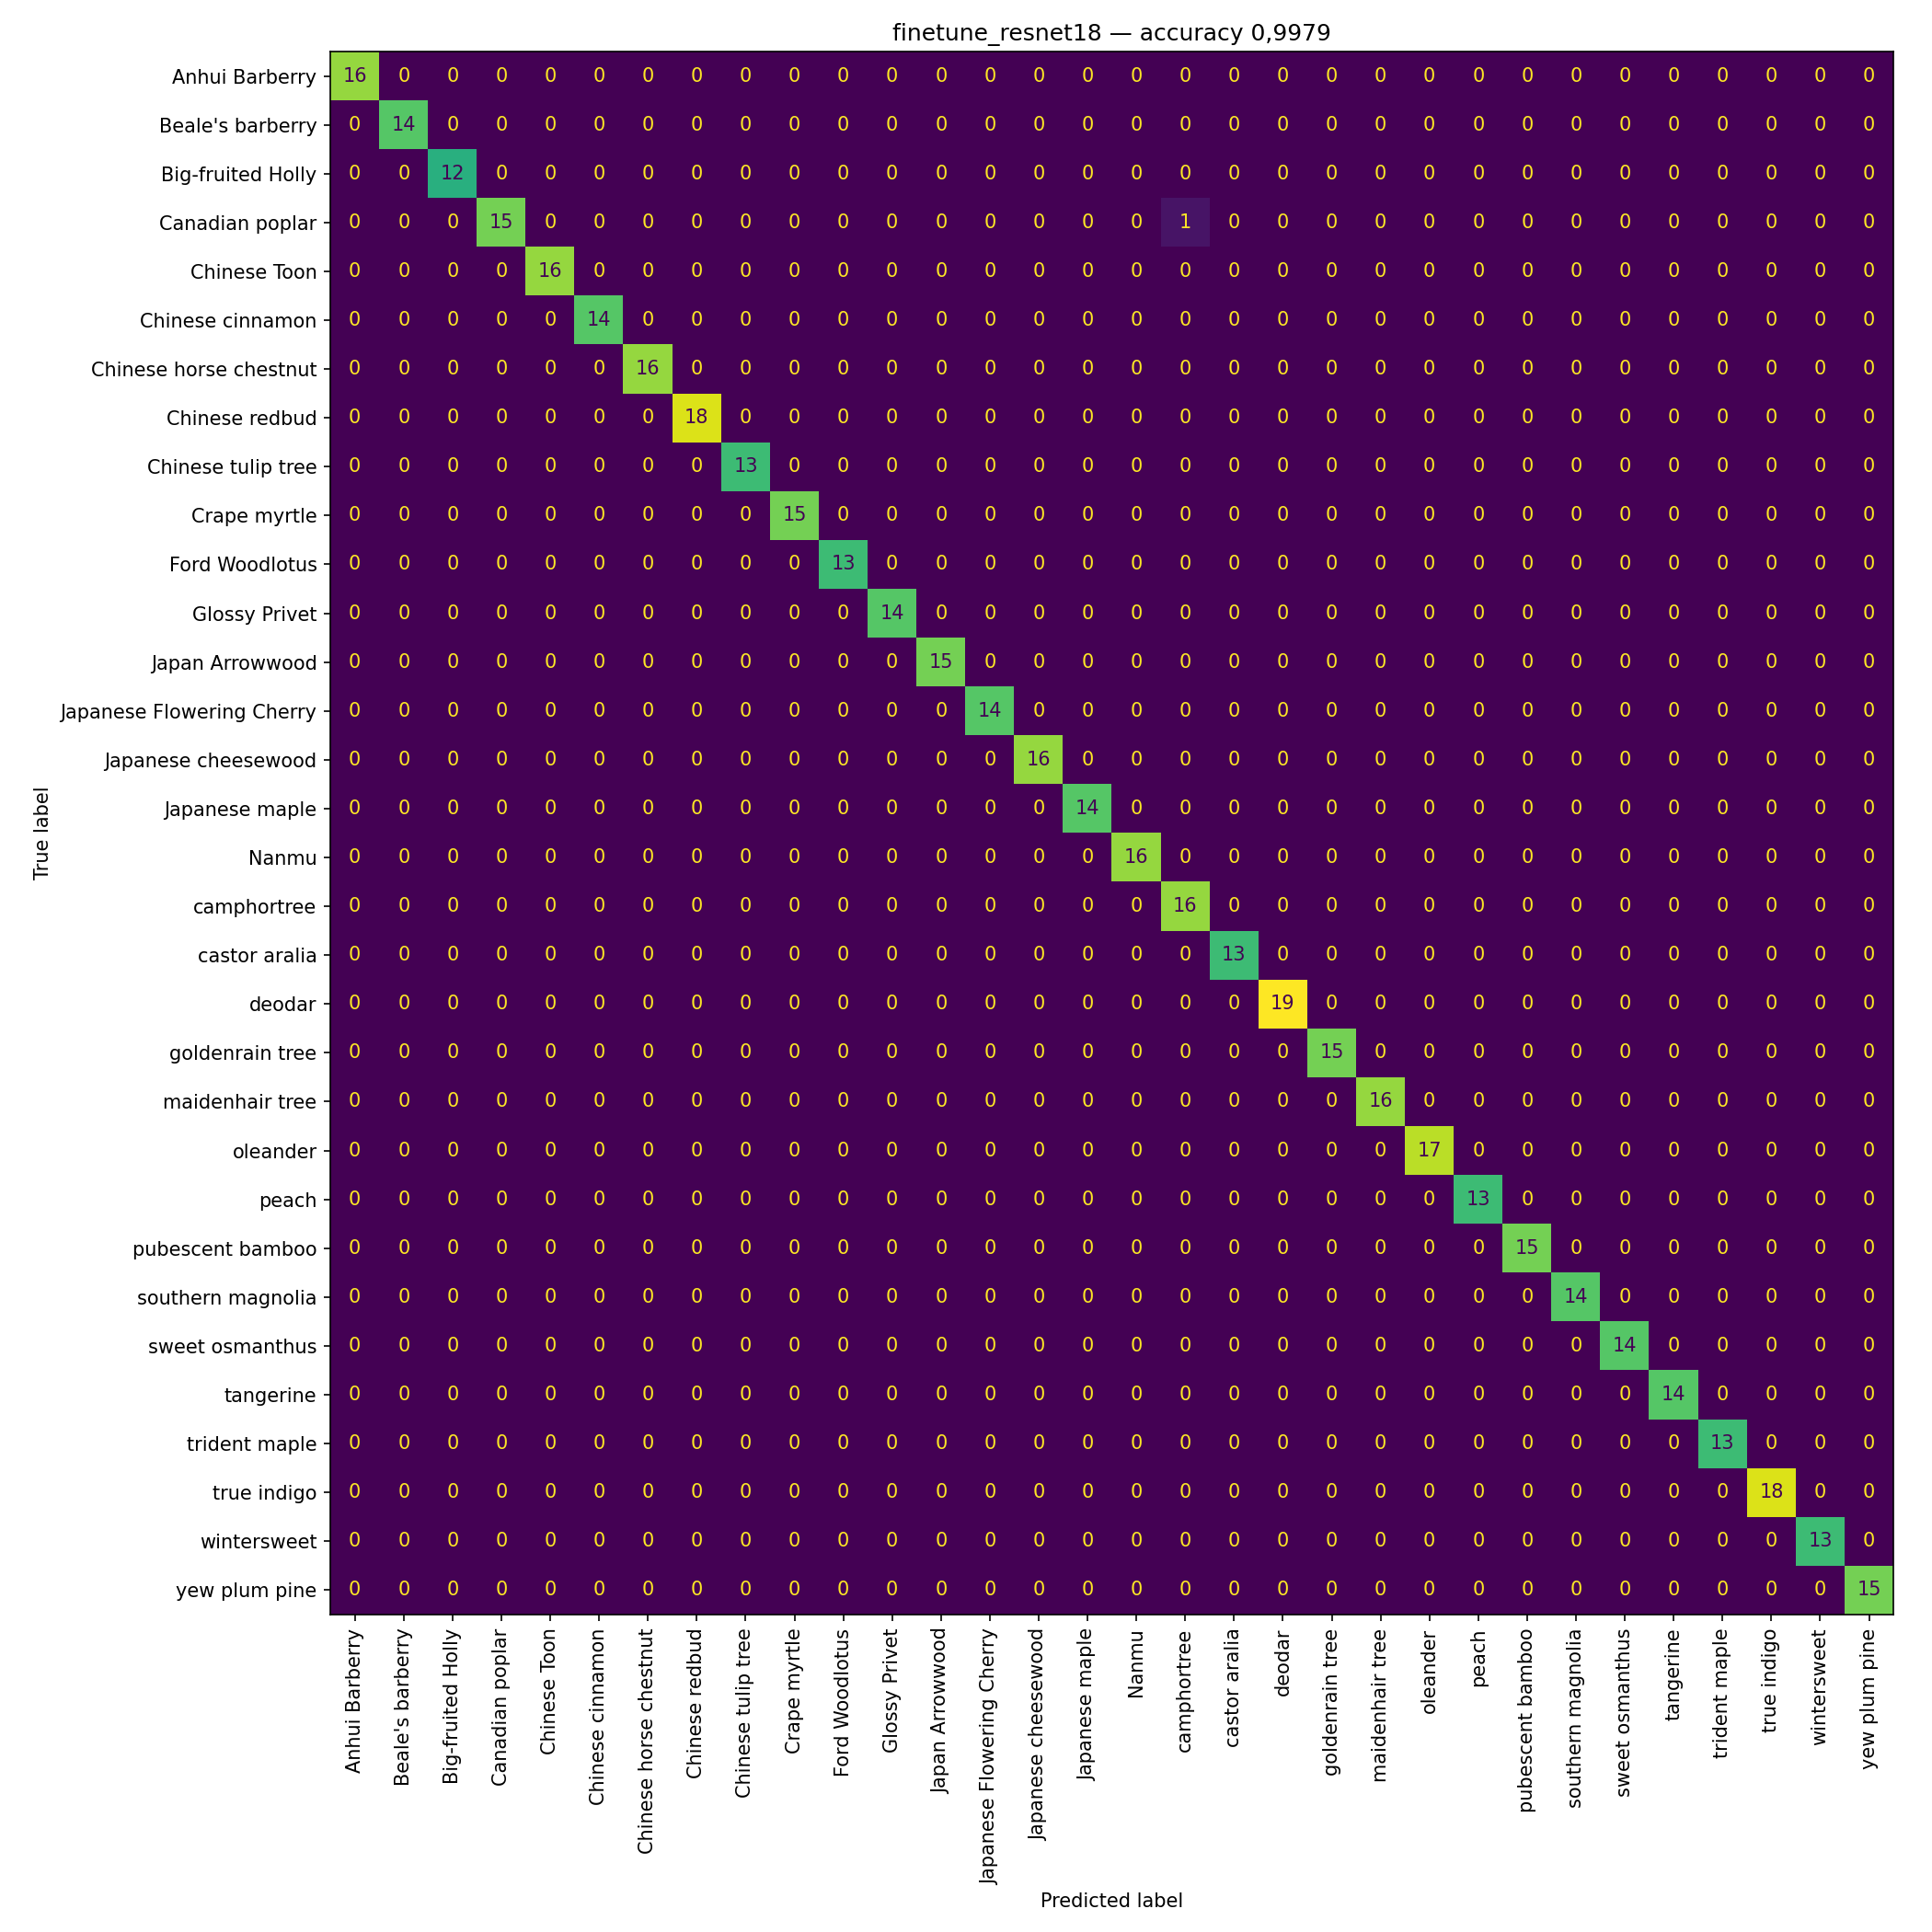
\includegraphics[width=0.82\linewidth]{confusion.png}
  \caption{Ma trận nhầm lẫn của mô hình ResNet18 tinh chỉnh trên 477 ảnh kiểm tra.}
  \label{fig:confusion}
\end{figure}

\section{Minh hoạ đặc trưng mà mạng học được}

Khác với đặc trưng thủ công --- nơi mỗi chiều có tên và công thức rõ ràng --- đặc trưng của CNN phải
được quan sát gián tiếp. Bốn góc nhìn dưới đây trả lời bốn câu hỏi khác nhau.

\textbf{Bộ lọc tầng đầu tiên} (Hình~\ref{fig:filters}) là 64 nhân $7\times7\times3$ hiển thị dưới
dạng ảnh màu. Có thể thấy rõ hai nhóm: các bộ lọc dò biên theo nhiều hướng (dạng sọc sáng tối) và
các bộ lọc đối lập màu (xanh--đỏ, xanh--vàng). Đây là những đặc trưng rất tổng quát, lý do khiến
tầng đầu có thể giữ nguyên khi chuyển sang bài toán lá cây.

\begin{figure}[t]
  \centering
  \begin{minipage}{0.36\linewidth}
    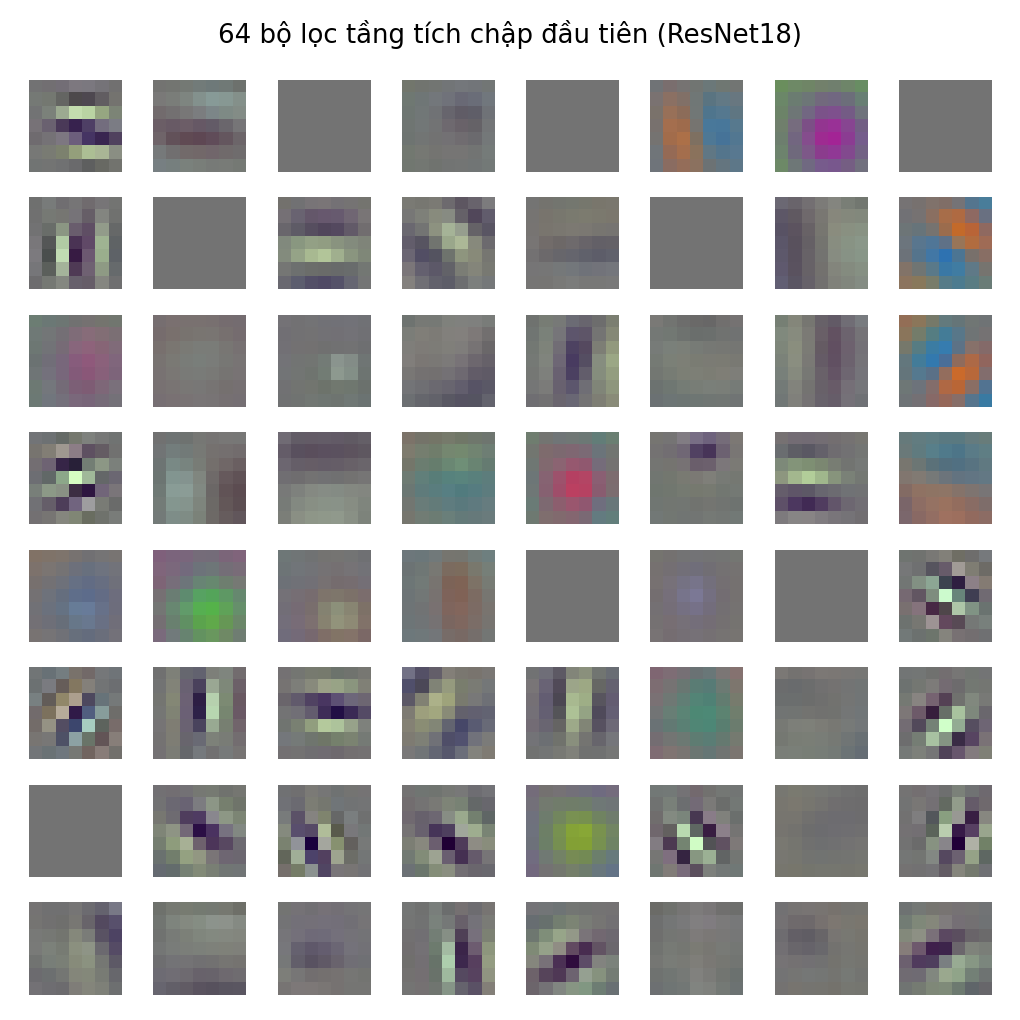
\includegraphics[width=\linewidth]{filters.png}
  \end{minipage}\hfill
  \begin{minipage}{0.62\linewidth}
    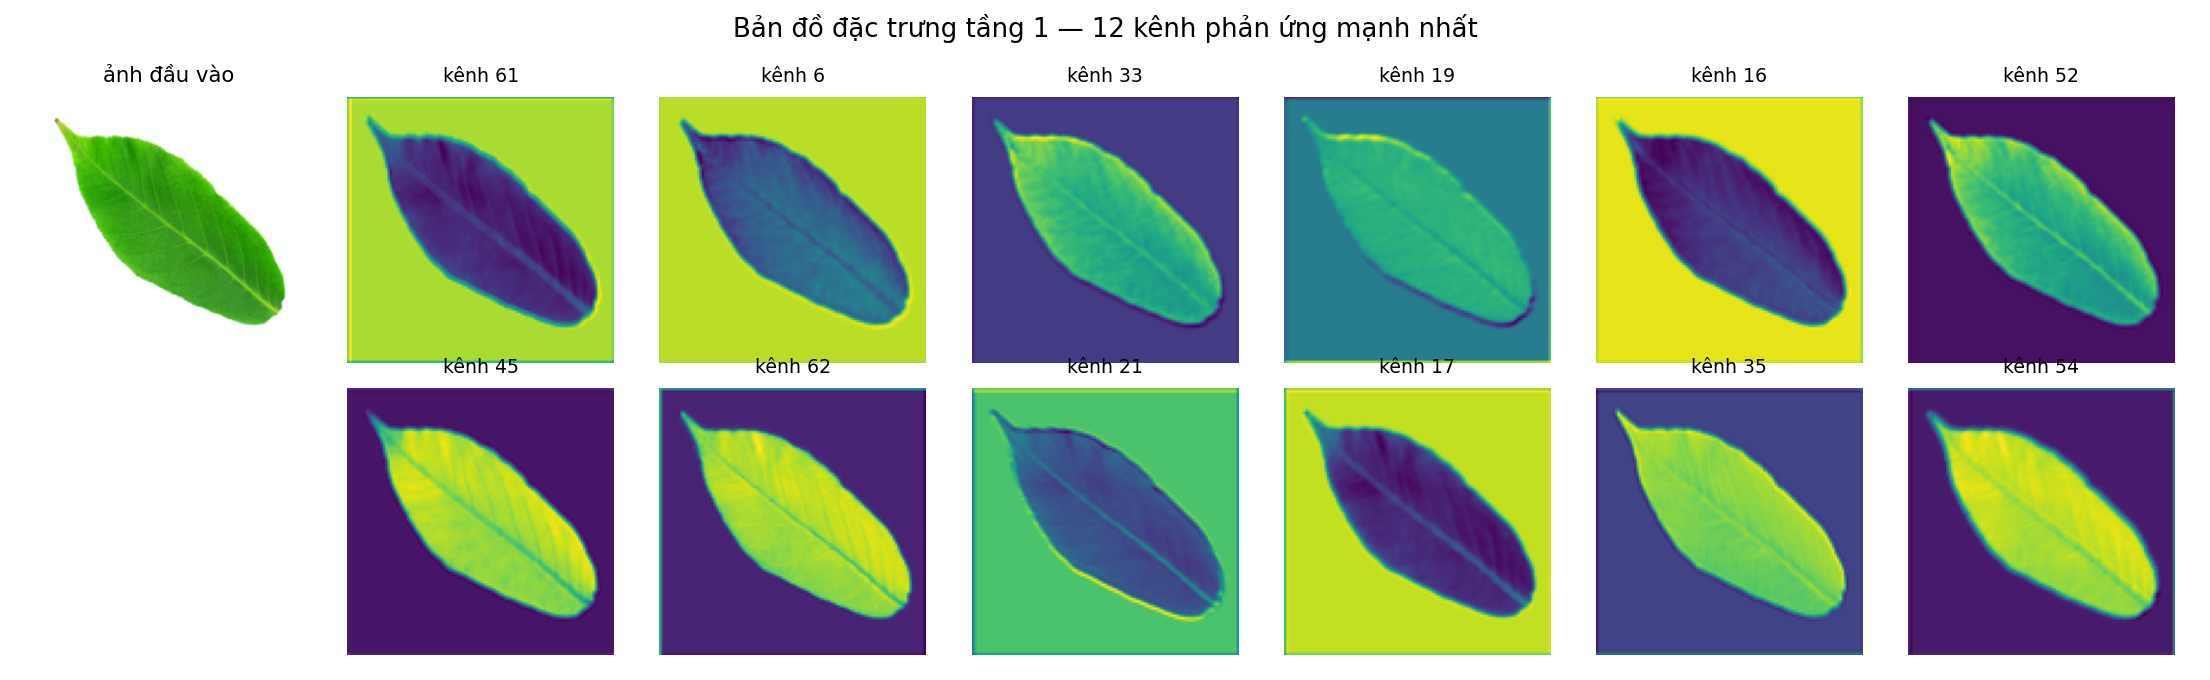
\includegraphics[width=\linewidth]{feature_maps.png}
  \end{minipage}
  \caption{Trái: 64 bộ lọc của tầng tích chập đầu tiên. Phải: bản đồ đặc trưng tương ứng trên một
  chiếc lá thật --- mỗi kênh làm nổi bật một loại cấu trúc khác nhau (mép lá, gân chính, vùng phiến lá).}
  \label{fig:filters}
\end{figure}

\textbf{Bản đồ đặc trưng} cho thấy những bộ lọc đó phản ứng thế nào trên một ảnh cụ thể: một số kênh
làm nổi mép lá, số khác làm nổi gân chính hoặc vùng phiến lá đồng nhất.

\textbf{Grad-CAM}~\cite{selvaraju2017} (Hình~\ref{fig:gradcam}) trả lời câu hỏi quan trọng nhất về
độ tin cậy: mạng dựa vào vùng nào để ra quyết định? Phương pháp lấy trọng số mỗi kênh của khối tích
chập cuối bằng gradient của điểm số lớp dự đoán theo kênh đó, rồi cộng lại. Bản đồ thu được tập
trung vào phiến lá và tắt dần ra nền, xác nhận mạng nhìn vào chiếc lá chứ không bám vào nền trắng
hay một dấu vết nào của máy quét. Đây là kiểm tra cần thiết: với nền trắng đồng nhất, một mô hình
vẫn có thể đạt độ chính xác cao nhờ học các manh mối giả.

\begin{figure}[t]
  \centering
  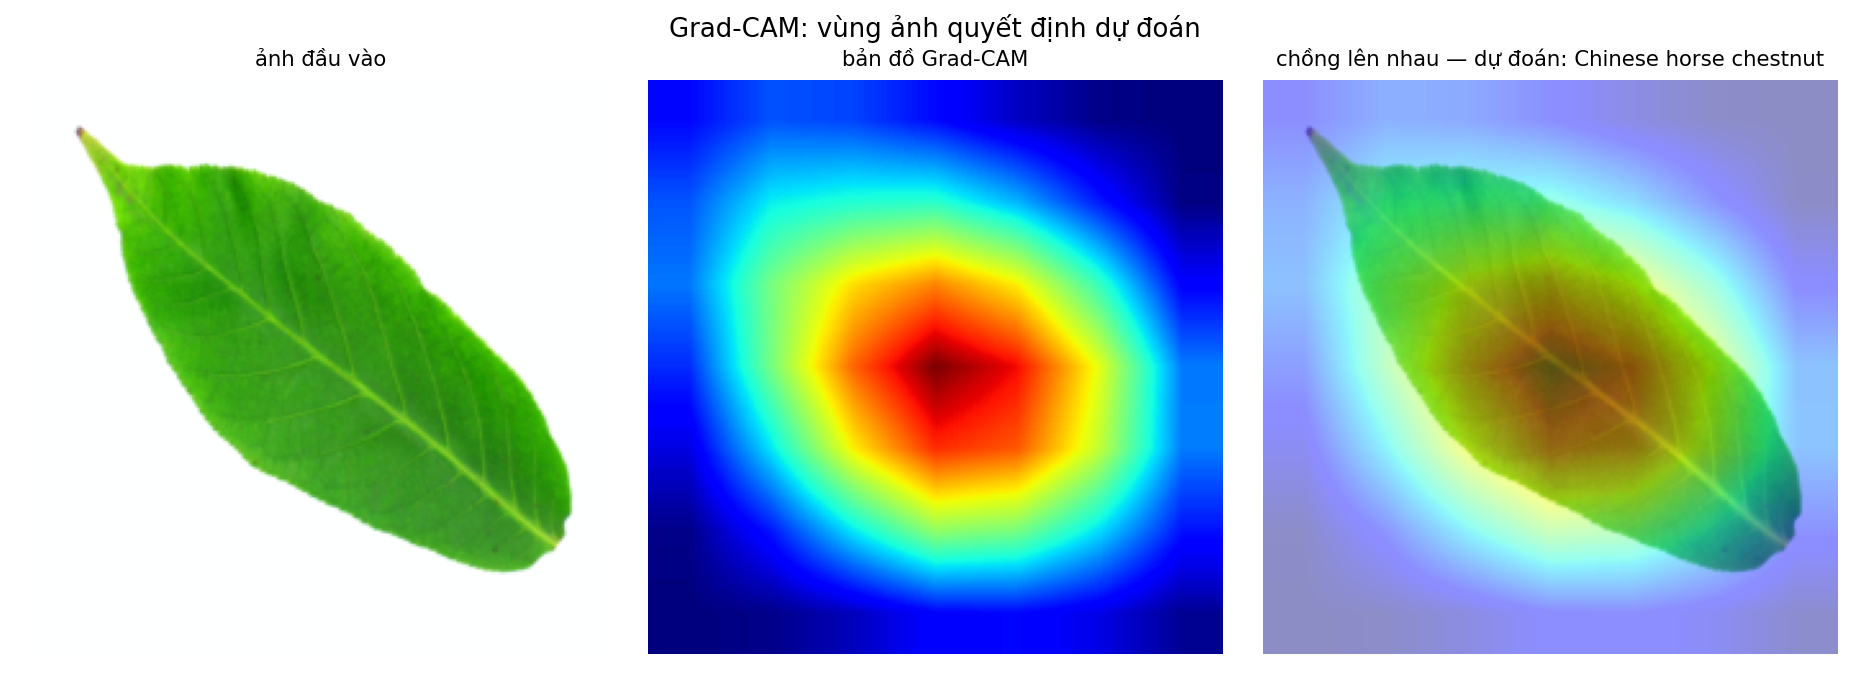
\includegraphics[width=\linewidth]{gradcam.png}
  \caption{Grad-CAM trên ảnh 1083. Vùng nóng nằm trọn trong phiến lá.}
  \label{fig:gradcam}
\end{figure}

\textbf{t-SNE}~\cite{maaten2008} (Hình~\ref{fig:tsne}) chiếu embedding 512 chiều của backbone đóng
băng xuống hai chiều. Các loài tách thành những cụm rời rạc \emph{trước khi} có bất kỳ bộ phân lớp
nào. Đây là lời giải thích trực quan cho kết quả ở Bảng~\ref{tab:backbones}: bộ phân lớp tuyến tính
đạt gần 100\% vì công việc khó đã được backbone làm xong.

So sánh với bài tập trước rất đáng chú ý: ở đó, phép chiếu hai chiều bằng PCA hay LDA đều \emph{không}
tách được các lớp, vì thông tin phân biệt nằm rải rác ở nhiều chiều. Với embedding của CNN, cấu trúc
cụm hiện rõ ngay trên hai chiều.

\begin{figure}[t]
  \centering
  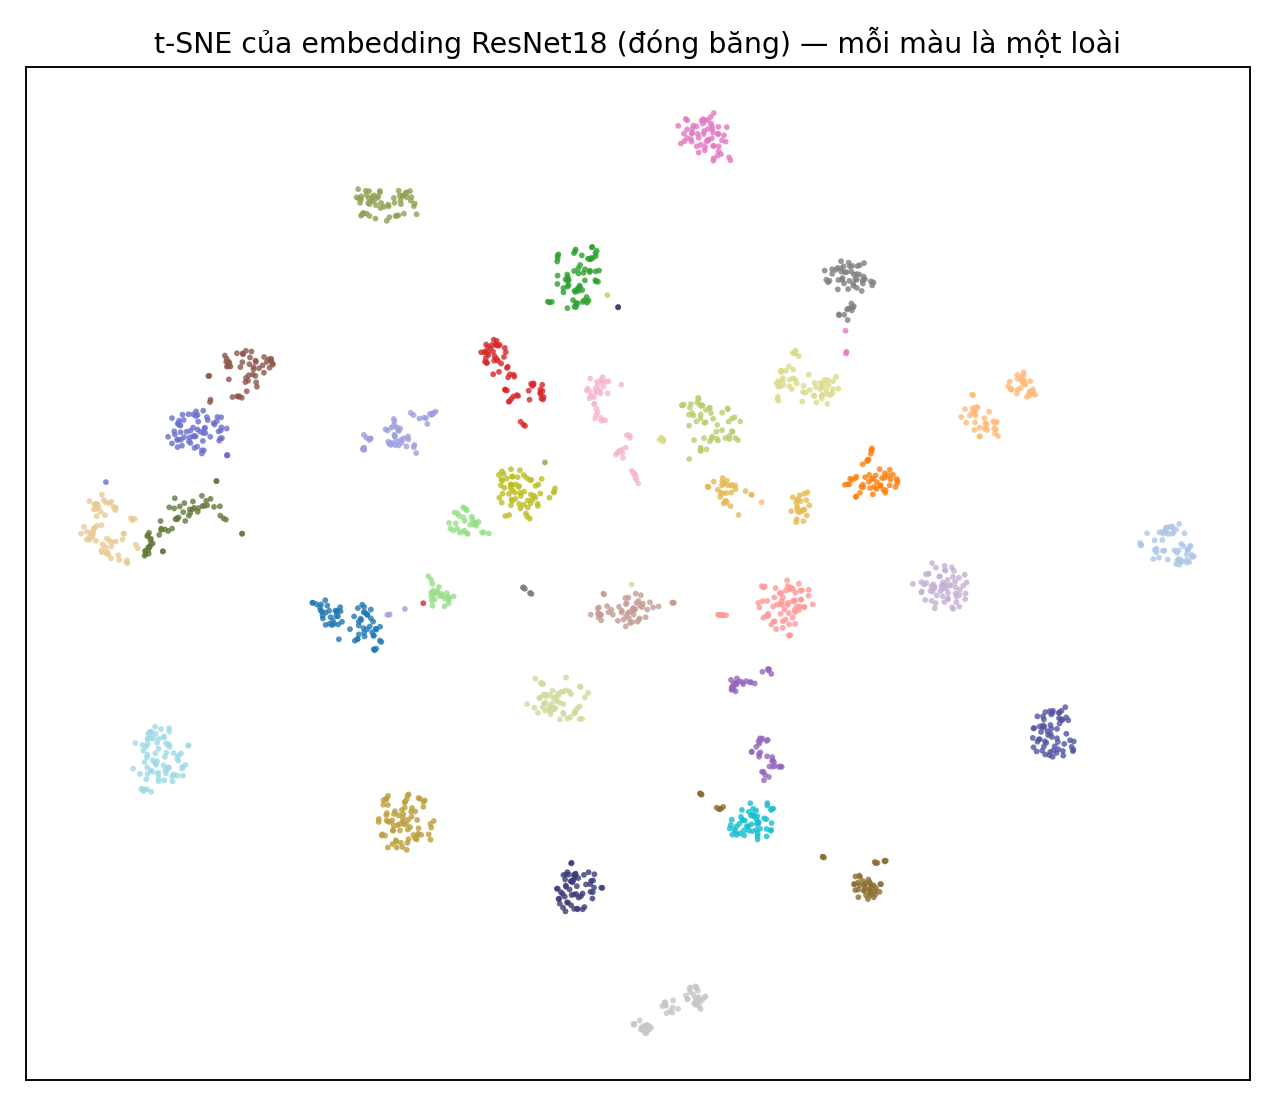
\includegraphics[width=0.68\linewidth]{tsne.png}
  \caption{t-SNE của embedding ResNet18 đóng băng; mỗi màu là một loài.}
  \label{fig:tsne}
\end{figure}

\section{Thảo luận: CNN so với đặc trưng thủ công}

Bảng~\ref{tab:comparison} đặt hai cách tiếp cận cạnh nhau. CNN thắng về độ chính xác, nhưng bức
tranh đầy đủ có nhiều chiều hơn một con số.

\textbf{Công sức thiết kế.} Quy trình thủ công cần bốn nhóm đặc trưng được thiết kế riêng, cộng với
một bước phân đoạn mà bài tập trước đo được là có lỗi cục bộ trên các lá có mặt dưới nhạt màu. Quy
trình CNN không cần bước nào trong số đó.

\textbf{Khả năng giải thích.} Ở chiều ngược lại, đặc trưng thủ công có thể nói chính xác vì sao mô
hình quyết định: bài tập trước định lượng được rằng \emph{smooth factor} là đặc trưng quan trọng
nhất, và đo được mức độ chồng lấn thông tin giữa nhóm màu và nhóm kết cấu. Với CNN, câu trả lời
tương đương chỉ có thể tiếp cận gián tiếp qua Grad-CAM.

\textbf{Chi phí tính toán.} Trích đặc trưng thủ công mất khoảng 0,27 giây mỗi ảnh trên CPU, trong
khi MobileNetV3 chỉ mất \lightms{} mili giây --- CNN hiện đại thực ra \emph{nhanh hơn} quy trình thủ
công, vì phép phân đoạn và các phép hình thái học trên ảnh $1600\times1200$ khá tốn kém. Bù lại, CNN
cần tải về trọng số tiền huấn luyện và phụ thuộc vào một khung học sâu~\cite{paszke2019}.

\textbf{Tính bền vững.} Bài tập trước chỉ ra tổ hợp đặc trưng thủ công tốt nhất lại rất dễ vỡ khi
ảnh bị nhiễu hoặc che khuất. Báo cáo này chưa lặp lại thí nghiệm đó cho CNN, nên không thể khẳng
định bên nào bền hơn; đó là hướng cần làm tiếp.

\section{Hạn chế}

\begin{itemize}
  \item Độ chính xác đã chạm trần của bộ dữ liệu: \ftacc{} tương ứng \fterrors{} ảnh sai trên 477.
        Ở mức này, mọi so sánh giữa các cấu hình đều nằm trong vùng nhiễu thống kê, và Flavia không
        còn đủ khó để phân biệt các phương pháp.
  \item Cấu hình tinh chỉnh chỉ được đánh giá trên một phép chia giữ lại, không chạy kiểm định chéo
        đầy đủ vì chi phí tính toán trên CPU.
  \item Siêu tham số (tốc độ học, số epoch, mức độ mở khoá) được chọn theo kinh nghiệm, chưa qua tìm
        kiếm có hệ thống.
  \item Chưa thử kiến trúc Transformer thị giác, vốn cần nhiều dữ liệu hơn hoặc kỹ thuật huấn luyện
        riêng để phát huy trên tập nhỏ như Flavia.
\end{itemize}

\section{Kết luận}

Học chuyển giao giải bài toán Flavia tốt hơn quy trình đặc trưng thủ công với công sức thiết kế ít
hơn hẳn: \probebestname{} đóng băng đạt \probebestcv{} và ResNet18 tinh chỉnh đạt \ftacc{} trên tập
kiểm tra giữ lại, so với \classicalcv{} của bài tập trước.

Kết quả có ý nghĩa nhất không phải con số cao nhất, mà là \emph{phần lớn thành tích đến từ trước khi
huấn luyện}. Một bộ phân lớp tuyến tính trên đặc trưng ImageNet đóng băng đã vượt toàn bộ quy trình
thủ công, và hình t-SNE cho thấy lý do: các loài đã tách thành cụm ngay trong không gian embedding.
Việc tinh chỉnh chỉ thêm được một phần nhỏ. Với một bộ dữ liệu 1907 ảnh, giá trị của học sâu nằm ở
biểu diễn được chuyển giao từ dữ liệu lớn, chứ không nằm ở việc huấn luyện trên chính bộ dữ liệu nhỏ đó.

Quan sát thứ hai là số tham số không phải chỉ dấu của chất lượng: \lightname{} nhỏ hơn \heavyname{}
\paramratio{} lần nhưng cho kết quả cao hơn và nhanh hơn 5 lần, đủ nhẹ để triển khai trên thiết bị
di động.

\begin{thebibliography}{99}

\bibitem{lecun1998}
Y.~LeCun, L.~Bottou, Y.~Bengio, and P.~Haffner, ``Gradient-based learning applied to document
recognition,'' \emph{Proceedings of the IEEE}, vol.~86, no.~11, pp.~2278--2324, 1998.

\bibitem{deng2009}
J.~Deng, W.~Dong, R.~Socher, L.-J. Li, K.~Li, and L.~Fei-Fei, ``ImageNet: A large-scale hierarchical
image database,'' in \emph{Proc. IEEE Conf. Computer Vision and Pattern Recognition (CVPR)}, 2009,
pp.~248--255.

\bibitem{krizhevsky2012}
A.~Krizhevsky, I.~Sutskever, and G.~E. Hinton, ``ImageNet classification with deep convolutional
neural networks,'' in \emph{Advances in Neural Information Processing Systems (NIPS)}, vol.~25,
2012, pp.~1097--1105.

\bibitem{simonyan2015}
K.~Simonyan and A.~Zisserman, ``Very deep convolutional networks for large-scale image
recognition,'' in \emph{Int. Conf. Learning Representations (ICLR)}, 2015, arXiv:1409.1556.

\bibitem{he2016}
K.~He, X.~Zhang, S.~Ren, and J.~Sun, ``Deep residual learning for image recognition,'' in
\emph{Proc. IEEE Conf. Computer Vision and Pattern Recognition (CVPR)}, 2016, pp.~770--778.

\bibitem{howard2019}
A.~Howard, M.~Sandler, G.~Chu, L.-C. Chen, B.~Chen, M.~Tan, W.~Wang, Y.~Zhu, R.~Pang, V.~Vasudevan,
Q.~V. Le, and H.~Adam, ``Searching for MobileNetV3,'' in \emph{Proc. IEEE/CVF Int. Conf. Computer
Vision (ICCV)}, 2019, pp.~1314--1324.

\bibitem{selvaraju2017}
R.~R. Selvaraju, M.~Cogswell, A.~Das, R.~Vedantam, D.~Parikh, and D.~Batra, ``Grad-CAM: Visual
explanations from deep networks via gradient-based localization,'' in \emph{Proc. IEEE Int. Conf.
Computer Vision (ICCV)}, 2017, pp.~618--626.

\bibitem{maaten2008}
L.~van der Maaten and G.~Hinton, ``Visualizing data using t-SNE,'' \emph{Journal of Machine Learning
Research}, vol.~9, pp.~2579--2605, 2008.

\bibitem{paszke2019}
A.~Paszke \emph{et al.}, ``PyTorch: An imperative style, high-performance deep learning library,'' in
\emph{Advances in Neural Information Processing Systems (NeurIPS)}, 2019, pp.~8024--8035.

\bibitem{wu2007}
S.~G. Wu, F.~S. Bao, E.~Y. Xu, Y.-X. Wang, Y.-F. Chang, and Q.-L. Xiang, ``A leaf recognition
algorithm for plant classification using probabilistic neural network,'' in \emph{Proc. IEEE Int.
Symp. Signal Processing and Information Technology (ISSPIT)}, 2007, pp.~11--16.

\end{thebibliography}

\end{document}
